\documentclass[10pt,letterpaper]{article}
\newif\ificmlstyle
\IfFileExists{icml2026.sty}{
  \icmlstyletrue
  \usepackage[accepted]{icml2026}
}{
  \usepackage[letterpaper,top=0.78in,bottom=0.77in,left=0.78in,right=0.78in,columnsep=0.29in]{geometry}
  \usepackage{times}
  \usepackage[round,authoryear]{natbib}
}
\usepackage[T1]{fontenc}
\usepackage{amsmath,booktabs,graphicx,microtype}
\graphicspath{{../figures/}}
\setlength{\textfloatsep}{10pt plus 3pt minus 3pt}
\setlength{\floatsep}{9pt plus 3pt minus 2pt}
\setlength{\dbltextfloatsep}{10pt plus 3pt minus 3pt}
\setlength{\intextsep}{9pt plus 2pt minus 2pt}
\setlength{\emergencystretch}{1.4em}
\newcommand{\papertitle}{From Camera Pose to Object Motion in Multi-View QA}
\newcommand{\people}{Ashman Mehra, Wen-Chi Tsai, Zhengfei Li, Mike Pupat}
\ificmlstyle
  \icmltitlerunning{Geometric Evidence for Multi-View QA}
\else
  \title{\vspace{-2.5em}\bfseries \papertitle}
  \author{\people\\[2pt]\small Carnegie Mellon University \enspace|\enspace 11-777 Project Checkpoint}
  \date{}
\fi
\begin{document}
\ificmlstyle
  \twocolumn[
  \icmltitle{\papertitle}
  \begin{icmlauthorlist}
  \icmlauthor{Ashman Mehra}{cmu}
  \icmlauthor{Wen-Chi Tsai}{cmu}
  \icmlauthor{Zhengfei Li}{cmu}
  \icmlauthor{Mike Pupat}{cmu}
  \end{icmlauthorlist}
  \icmlaffiliation{cmu}{Carnegie Mellon University}
  \vskip .3in
  ]
  \printAffiliationsAndNotice{11-777 Project Checkpoint, Fall 2026.}
\else
  \twocolumn[\maketitle]
\fi
\begin{abstract}
A change between two images can come from object motion, a new camera viewpoint, or both. We study how to make geometric evidence usable for multi-view vision-language question answering. On 1,000 MMSI-Bench questions, geometry-supervised adaptation with continuous camera hints improves Qwen3-VL from 30.2\% to 35.3\% and 34.6\% across two seeds, while accuracy on multi-image reasoning falls. On 24 controlled MOVi pairs, a reader given verified evidence answers both reference-frame questions correctly in all 24 pairs after explicit routing and thresholding, compared with 8 pairs when given coordinates for both frames. On 48 further MOVi scenes, a frozen grounder answers image motion correctly in 46 cases and scene motion in 29, with 14 of 36 moving targets called still. These controls isolate how the reader uses evidence and show where obtaining reliable evidence remains difficult.
\end{abstract}

\section{Introduction}
Two images of the same scene can tell different stories about motion. In Figure~\ref{fig:cable}, a cable appears to move left because the camera changes viewpoint. The image answer is \emph{left}, while the scene answer is \emph{still} under the specified horizontal tolerance. A vision-language model (VLM) needs to link the target phrase to the same instance in both images, separate camera and object motion, and interpret the reference frame requested in the question.

The midterm supplied a frozen VLM with estimated camera pose. The method helped where the pose nearly supplied the answer, and object-related categories had mixed results. We extend that idea with two implementations of geometric evidence: an adapted VLM for general benchmark QA and an explicit grounder for named-object motion. The first measures benchmark accuracy. The second permits controlled substitutions of object and camera evidence, which helps identify where an answer fails.

\begin{figure}[t]
  \centering
  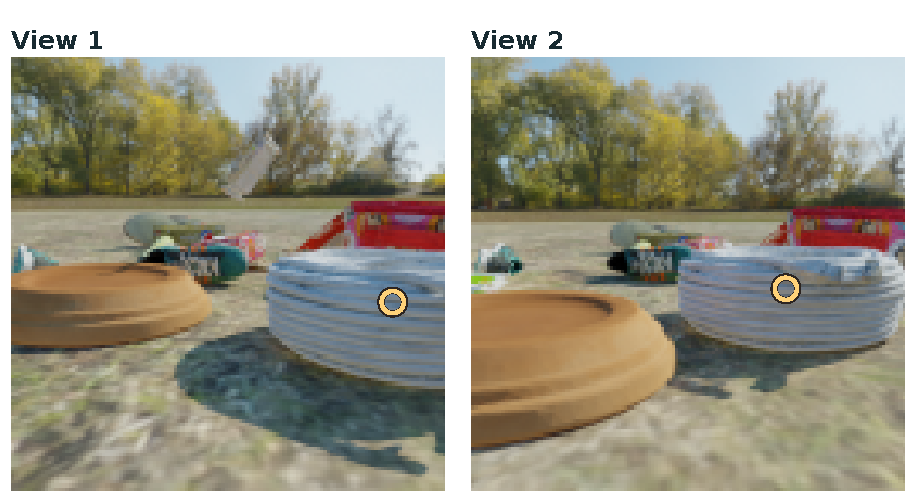
\includegraphics[width=.87\columnwidth]{cable_pair.pdf}
  \caption{One MOVi-E pair (scene 36). Rings show verified projections of the cable's center. The image center moves left by 0.154 image widths. Horizontal scene displacement in the first camera's coordinates is $-0.008$ simulator units, within the still tolerance.}
  \label{fig:cable}
\end{figure}

\section{Related Work}
MMSI-Bench evaluates spatial relationships across images \citep{yang2025mmsi}. SAT uses spatial supervision to train multimodal models \citep{ray2024sat}. We use spatial data for adaptation and use external controls to distinguish evidence extraction from evidence use. For geometric evidence, VGGT jointly predicts camera parameters and 3D structure \citep{wang2025vggt}. We compare ways of getting that geometry into Qwen VLMs \citep{bai2025qwen25vl,bai2025qwen3vl}, including low-rank adaptation \citep{hu2022lora}. Referring video segmentation links language to an instance over time \citep{khoreva2019ref}; our controls use CLIPSeg, SAM~2, and RAFT to distinguish referred-object localization from correspondence and 3D lifting \citep{luddecke2022clipseg,ravi2024sam2,teed2020raft}. Kubric's simulated scenes provide the poses and centers needed for verified motion evidence \citep{greff2022kubric}.

\section{Problem and Evaluation}
A benchmark item contains images $\mathcal I$, a question $q$, four options and the gold answer $y$. We measure mean exact-choice accuracy, $\frac1N\sum_i \mathbf{1}[\hat y_i=y_i]$, within the specified evaluation cohort. For controlled motion, $\mathcal I=(I_1,I_2)$ and $q$ names an object and specifies the reference frame. The two views yield two gold labels, $y_{\mathrm{img}}$ and $y_{\mathrm{scene}}$, each from $\{\mathrm{left},\mathrm{still},\mathrm{right}\}$. Pair accuracy requires both labels to be correct.

\paragraph{Dataset roles.}
MMSI-Bench supplies 1,000 multi-image questions across 11 categories for evaluation. The Qwen2.5-VL follow-up uses a targeted 423-question subset. SAT training images and questions supply supervision for the benchmark model. Ref-DAVIS17 provides real video, first-frame referring expressions and instance masks for measuring horizontal image motion and target-mask intersection over union (IoU). For the Ref-DAVIS17 primary evaluation we use 120 saved examples from official validation, with 40 per direction label and 30 videos. We use two different MOVi controls for this report: 24 pairs with a balanced set of image--scene relationships, and 48 disjoint scenes with 12 targets in each absolute scene-motion band (still, small, moderate, large). The latter favors visible, identifiable targets and has equal counts in each moving direction within each band. Each fresh scene contributes one named object and one pair.

\section{Geometric Evidence}
\paragraph{Pose hints and adaptation.}
The midterm decoded camera centers and viewing directions from VGGT and expressed motion relative to view~1 as continuous text. The adapted method creates additional spatial QA examples by localizing objects with frozen Qwen3-VL, using VGGT point maps to lift the localizations, and deriving camera--object and object--object answers geometrically. The principal training mixture contains 1,800 SAT motion examples and 1,800 geometry-derived examples. We fit rank-16 LoRA adapters with answer-token cross-entropy while keeping the base weights frozen. We compare the adapted model with and without pose text at test time, alongside raw and pose-text-only frozen baselines. Inputs to the presented adapted-plus-pose condition are images, the question, options, and continuous pose text. The geometry-derived training examples can teach object-relative relationships even though the test hint itself describes camera pose.

\paragraph{Explicit object grounding.}
For diagnostic motion QA, v2 uses per-view candidate localization and crop verification with Qwen3-VL, SAM~2 mask propagation, and RAFT surface correspondences. The pipeline uses VGGT depth and camera pose, background alignment and a visible-surface 3D estimator, with silhouette medians as a fallback. It uses unmarked images and a target phrase. This branch relies on pretrained modules and a fixed readout. Figure~\ref{fig:method} shows the flow.
\begin{figure}[t]
  \centering
  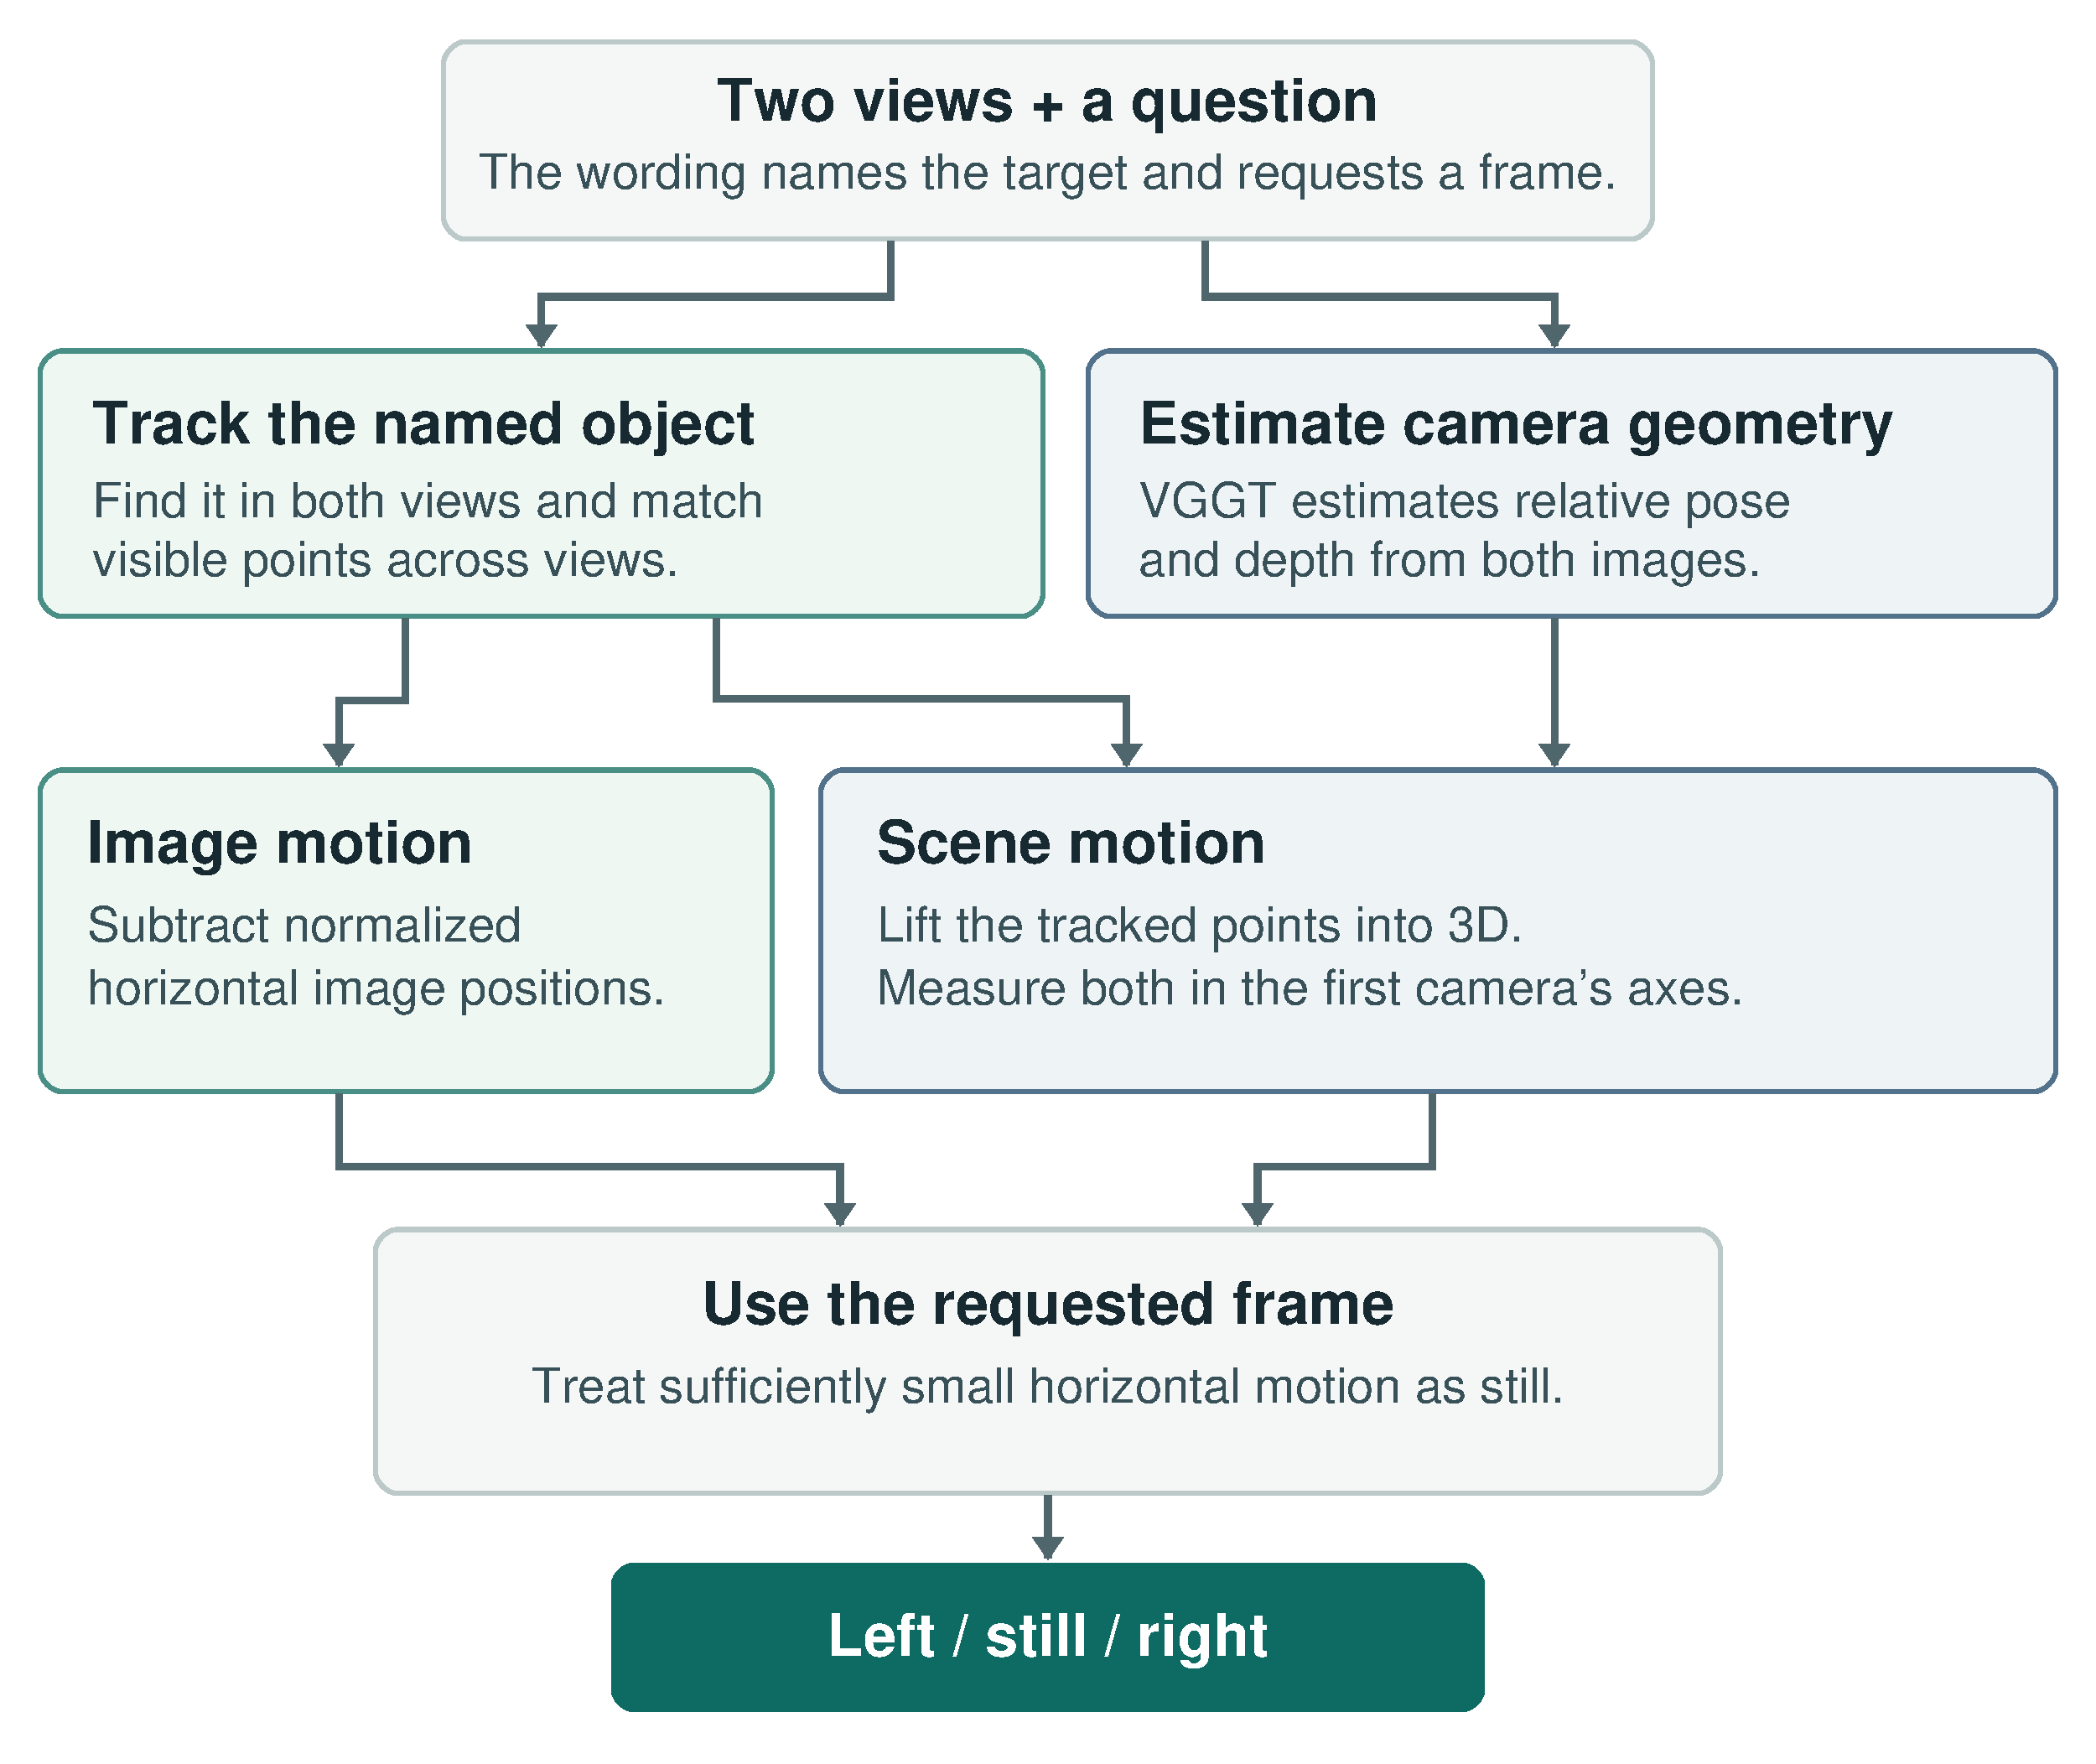
\includegraphics[width=.88\columnwidth]{grounding_pipeline.pdf}
  \caption{Explicit object-grounding branch. The image answer uses a change in projected position. The scene answer transforms a lifted point into the first camera's axes before measuring horizontal change.}
  \label{fig:method}
\end{figure}

\paragraph{Reference-frame readout.}
Let $u_i$ be the normalized horizontal image position in view $i$, and $\mathbf p_i$ a 3D point in camera $i$ coordinates. With $\mathbf p_2=R_{21}\mathbf p_1+\mathbf t_{21}$ for a static point, the two candidate displacements are
\begin{align}
 \Delta u &= u_2-u_1,\\
 \Delta x &= [R_{21}^{\top}(\mathbf p_2-\mathbf t_{21})-\mathbf p_1]_x.
\end{align}
Positive values point right. The reader outputs still when $|\Delta|\le\epsilon$ and otherwise uses the sign. The MOVi image tolerance is 0.02 image widths. The scene tolerance is 0.05 in the corresponding scene-coordinate system. For model evidence, coordinates are scaled so VGGT's median first-view depth is 5, giving canonical units. Simulator labels use 0.05 simulator units. In the routed Qwen condition, a text router chooses the reference frame and a deterministic step sets in-band displacements to exact zero before Qwen reads them. We also measure the deterministic answer alone.

\section{Results}
\subsection{When Do Pose and Adaptation Improve QA?}
The submitted Qwen2.5-VL midterm went from 26.5\% to 30.0\% overall when pose text was added (paired 95\% interval $[-0.1,7.1]$ percentage points, exact McNemar $p=.065$). Camera motion rose from 14.9\% to 37.8\% ($n=74$, $p=.001$). Object motion fell from 30.3\% to 25.0\% in this comparison. The text-only trace judge had limited overall discrimination between correct and incorrect answers.

In the full Qwen3-VL evaluation with direct decoding, 30.2\% raw becomes 32.7\% with continuous pose text. Adaptation without test-time geometry gives 32.8\% and 30.3\%. Adaptation plus pose text gives 35.3\% and 34.6\% (Figure~\ref{fig:mmsi}). The paired gains over raw are 5.1 points (95\% CI $[2.0,8.3]$, $p=.0034$) and 4.4 points ($[1.0,7.6]$, $p=.0158$). Both full-cohort intervals against pose hints alone cross zero. Accuracy on object--object questions falls (24.5\% and 25.5\% versus 30.9\% raw, $n=94$). On 198 multi-image reasoning items, the adapted-plus-pose model drops from 36.4\% to 28.3\% and 26.3\%. Most examples in this category have three or more views, so two-view adaptation is a plausible contributor to the regression.
\begin{figure}[t]
  \centering
  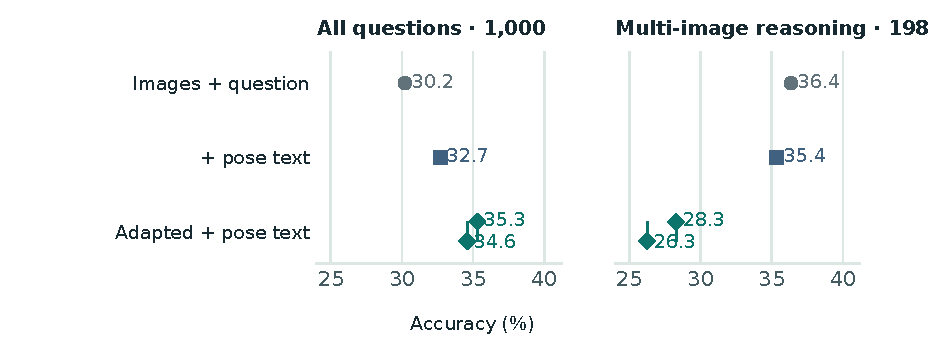
\includegraphics[width=\columnwidth]{mmsi_headlines.pdf}
  \caption{Matched Qwen3-VL direct evaluation. All conditions see the same items within each panel. The two adaptation points are seeds 42 and 123.}
  \label{fig:mmsi}
\end{figure}

The 423-item direct Qwen2.5-VL run gives 30.0\% raw, 31.9\% with pose hints, 33.1\% adapted without hints, and 35.0\% adapted with hints. Camera--object rises from 22.1\% with hints alone to 40.7\% after adaptation. This comparison checks a second Qwen backbone. The midterm retains its original prompt and evaluation settings. On the 329-item Qwen3-VL core subset, a discrete geometry tool scores 23.1\% against 33.4\% for continuous pose text. Binning can discard pitch and larger rotations. These sequential benchmark explorations serve as comparisons across existing conditions.

\subsection{Can the Reader Use Correct Object Evidence?}
On Ref-DAVIS17, CLIPSeg and Qwen3-VL remain frozen. A learned matching head fits two weights and a bias to combine phrase-conditioned target evidence with cosine similarity to a source-frame foreground prototype. We compare with a matched independent head using a target-frame prototype and a fixed-weight source-matching head. The learned and independent heads use 847 training rows and minimize binary cross-entropy plus Dice loss. The four-arm comparison in Table~\ref{tab:davis} shows that coordinates improve QA over raw while fitting the source link provides little further gain. The learned-minus-independent IoU gain is 0.0013 with a paired video-bootstrap 95\% interval of $[-0.0008,0.0041]$. On unchanged items, applying the 0.10-image-width rule to the learned head's coordinates gives 24/40 correct, whereas Qwen reading those same coordinates gives 2/40. All 120 intended primary items are present in the archive. The combined primary and secondary-swap completion flag remains false, and this experiment stopped at external validation.
\begin{table}[t]
\centering\small
\caption{Ref-DAVIS17 primary results. There are 40 examples per class, so balanced and raw accuracy coincide. IoU compares the predicted and verified target masks.}
\label{tab:davis}
\begin{tabular}{lrr}
\toprule
Condition & Correct / 120 & Mean IoU \\
\midrule
Images + question & 45 & -- \\
Independent localization & 64 & .3721 \\
Fixed correspondence & 65 & .3709 \\
Learned correspondence & 64 & .3734 \\
\bottomrule
\end{tabular}
\end{table}

On the 24 reference-frame-balanced MOVi pairs, Qwen answers both questions correctly on 2/24 pairs with images alone. With verified coordinates for both frames it gets 8/24, and coordinates for just the requested frame give 12/24. Routing and applying the still tolerance before Qwen reads the displacement gives 24/24 verified and 17/24 with predicted v2 evidence. Deterministic readout gives the same predicted-evidence answers in this cohort. The language router correctly routes all 48 questions with these templates. The routed comparison measures a system that performs the threshold decision before generation.

\subsection{Where Does Predicted Evidence Fail?}
On the 48 fresh MOVi scenes, the deterministic reader gets all 48 pairs with verified evidence. With frozen v2 evidence, it gets 46/48 image answers, 29/48 scene answers, and 29/48 complete pairs. V2b, a variant with a flow--mask agreement check, gives identical predictions on this fresh set. V2 called 14 of 36 movers \emph{still}, including 8/12 small, 5/12 moderate, and 1/12 large movements. It recognized 9/12 true-still targets, and 9/23 of its predicted-still answers were correct. These are cohort-specific rates.
\begin{figure}[t]
  \centering
  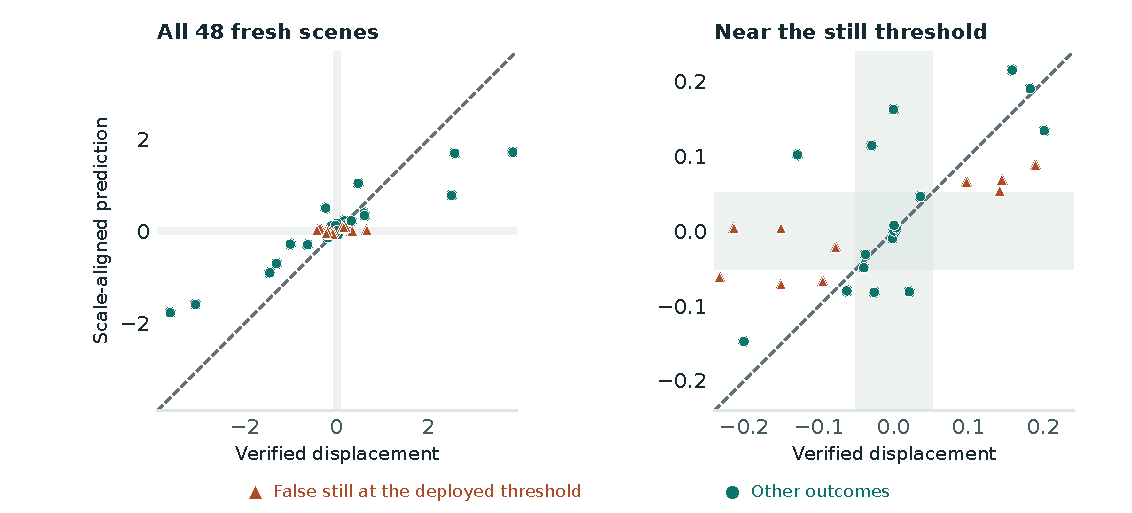
\includegraphics[width=\columnwidth]{displacement_audit.pdf}
  \caption{Fresh MOVi displacement after offline scale alignment. Shading shows the $\pm0.05$ simulator tolerance. Orange triangles indicate false still in deployed canonical units, so some can fall outside the shaded band after rescaling.}
  \label{fig:scatter}
\end{figure}

Reducing the canonical scene threshold from 0.05 to 0.02, with the candidate fixed before fresh inference, changes pair accuracy from 29/48 to 32/48 (six wins, three losses). It recovers seven moving directions and reduces true-still recall from 9/12 to 6/12. One false still changes to the wrong direction. The candidate misses the pre-set preservation criterion, which favors retaining the 0.05 threshold in the checkpoint.

\paragraph{Scale and center diagnostics.}
For Figure~\ref{fig:scatter}, we rescale v2 predictions offline using verified simulator axial depth. Magnitude is then smaller than truth for 31/36 movers, with median predicted-to-verified magnitude ratio 0.53. At the deployed scale, seven movers have the wrong sign, including four with static cameras. Substituting verified centers into the scale-aligned estimate yields 46/48 correct scene labels, whereas substituting verified pose yields 34/48 and scale alignment alone yields 35/48. A center substitution also supplies identity and depth, and substitutions can compensate for another error. These comparisons motivate investigating center lifting and surface selection. The model measures visible surface points while the simulator labels the center of mass, so changes in visible surface and object rotation can affect the estimates. Figure~\ref{fig:cases} shows examples.

\section{Conclusion and Limitations}
Geometry-derived training plus pose text improves overall benchmark QA under the matched Qwen3-VL setup, with losses in multi-image reasoning and object--object categories. Controlled object-motion questions expose two different problems. The VLM struggles to apply the reference-frame and still rules to coordinates without an explicit interface. The grounder can produce useful image coordinates while underestimating actual scene motion. Our explicit evidence is for two views, one named target, and horizontal motion. MOVi uses selected, low-resolution simulated images, and the scale and component swaps use privileged annotations. Future experiments could evaluate better center estimates under occlusion and rotation, and test multi-view training or a selective adapter. Transfer of the explicit grounder to general benchmark QA remains a separate experiment.

\ificmlstyle
  \IfFileExists{icml2026.bst}{\bibliographystyle{icml2026}}{\bibliographystyle{plainnat}}
\else
  \bibliographystyle{plainnat}
\fi
\bibliography{references}

\appendix
\section{Additional Ablations and Case Examples}
\label{app:figures}
Figure~\ref{fig:categories} gives the eleven MMSI-Bench category differences. Figure~\ref{fig:reader} shows the reader staircase. Figure~\ref{fig:threshold} compares both fresh thresholds on the same pairs. Removing surface flow gives 27/48 pairs and using raw VGGT pose gives 28/48. In the latter ablation the inter-view scale correction also changes on moving cameras.

\paragraph{Cohort details.}
Fresh MOVi scenes are disjoint from both archived 24-pair manifests. The selection uses 128-pixel images with at least 100 visible target pixels per view, image-edge and threshold-margin exclusions, and fixed bands on verified horizontal scene displacement. Small movers are above 0.05 and at most 0.20 simulator units, moderate movers are above 0.20 and at most 0.50, and large movers are above 0.50. The smaller 24-pair reader cohort tests camera-only motion, following a moving object, opposite image and scene directions, and agreement, with six pairs each. These cohorts serve different tests.

\begin{figure*}[p]
  \centering
  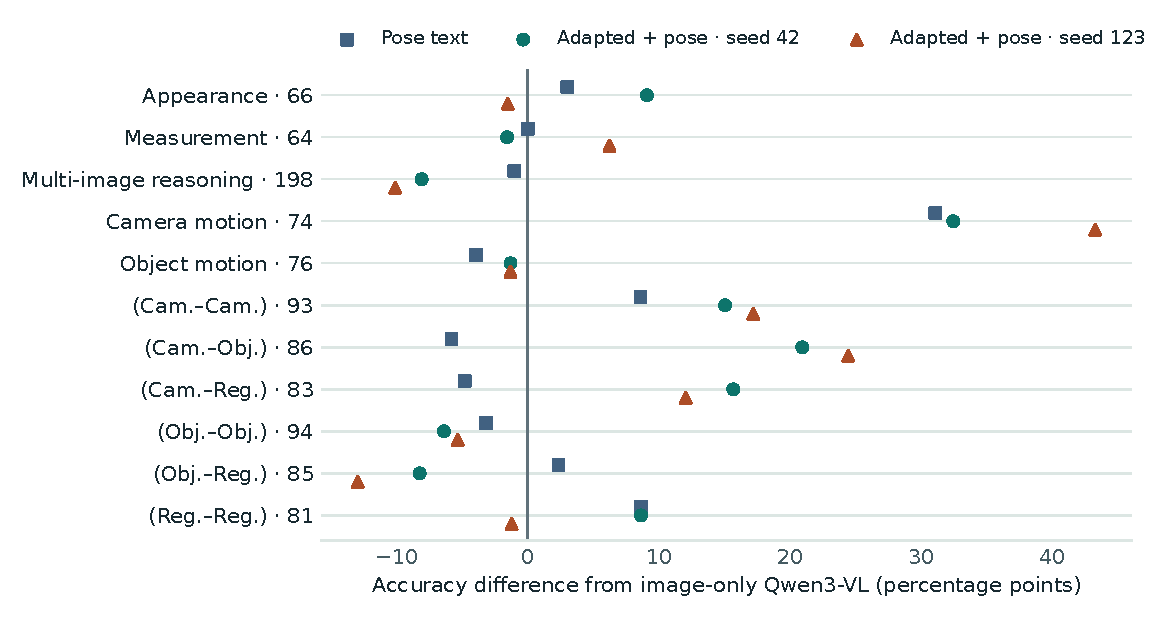
\includegraphics[width=.88\textwidth]{mmsi_categories.pdf}
  \caption{MMSI-Bench category differences from raw Qwen3-VL. The suffix on each row gives its denominator.}
  \label{fig:categories}
  \vspace{.16in}
  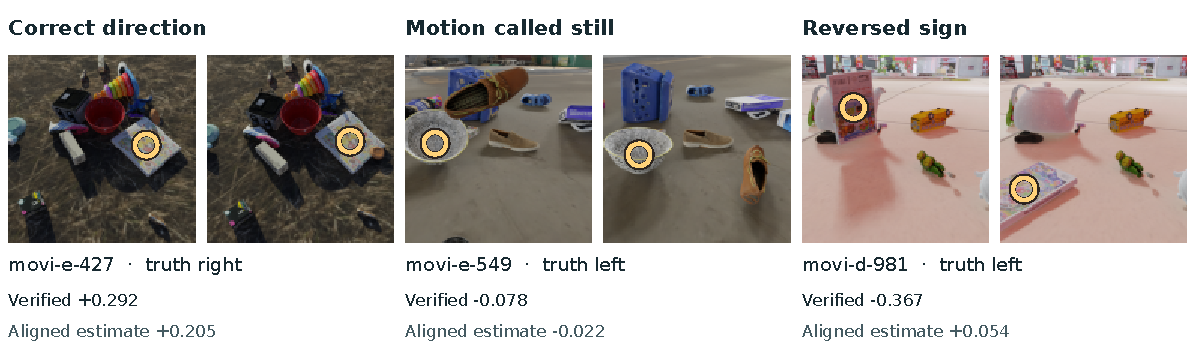
\includegraphics[width=.95\textwidth]{motion_examples.pdf}
  \caption{Fresh examples with verified projected centers marked. Displacements share simulator units after offline scale alignment. The middle estimate retains the sign but falls inside the tolerance. The right example reverses sign.}
  \label{fig:cases}
  \vspace{.17in}
  \begin{minipage}[t]{.49\textwidth}
    \centering
    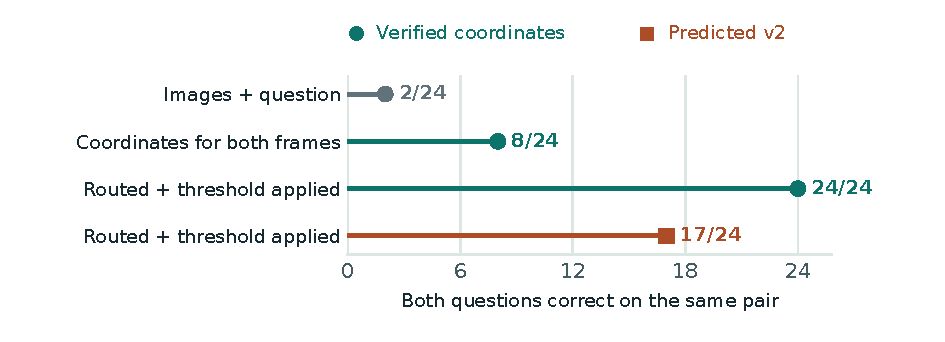
\includegraphics[width=\linewidth]{reader_interface.pdf}
    \caption{Both answers correct on each of the same 24 controlled MOVi pairs. Routed Qwen and deterministic readout match on all 48 answers with v2 evidence.}
    \label{fig:reader}
  \end{minipage}\hfill
  \begin{minipage}[t]{.49\textwidth}
    \centering
    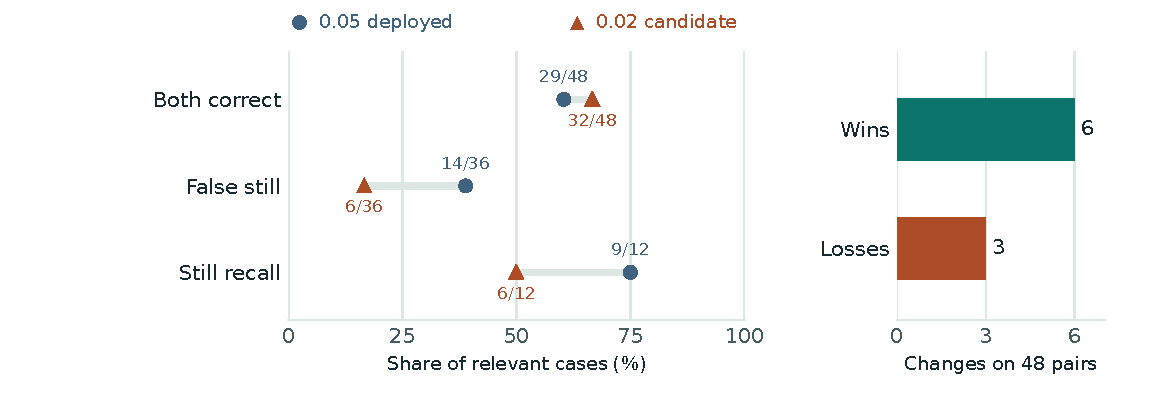
\includegraphics[width=\linewidth]{threshold_tradeoff.pdf}
    \caption{The 0.02 candidate improves pair accuracy while hurting still recall. Wins and losses count pair-level changes relative to 0.05.}
    \label{fig:threshold}
  \end{minipage}
\end{figure*}

\paragraph{Reproduction.}
The checkpoint's evidence ledger identifies frozen conditions and source files. The scripts verify condition totals and primary-cohort keys, then rebuild figures from archived scores and selected RGB frames on CPU. The ledger gives the thresholds and source conventions needed to reproduce each comparison.
\end{document}
